
\section{Introduction}


\subsection{Motivation}
% Choice overload
% Aktuelle Situation in der Kleidungsbranche
% kurzer Einblick in Recommender systems (wird spaeter weiter ausgefuehrt)
When a typical customer enters a shop or department store, he often gets confronted with a very large amount of products he can choose from.
This is especially true, when searching for products online on a web shop.
The commonly well-known web shop \gls{amazon.com} for instance, provides about 280 million different products on their internet presence solely for the United States - there are even more products offered world wide.\citep{marketplaceanalytics:2014}
Even shops dedicated to only a special kind of product can have a wide array of products.
On \gls{zalando}, a German online shop dedicated to clothing, one can choose out of 150.000 products and 1.500 different brands.\citep{visser:2014}\\

%\paragraph{Choice Overload}
\index{Choice Overload}
There is a general belief that great choice pleases the customers needs.
However it is actually proven, that this idea is not fully correct and reality is much more complex.
Already in 2000 a group of scientists demonstrated that a great variety can also have negative effects.
It is proven, that large assortments can lower the customers willingness to purchase products.\citep[p.~312-313]{diehl:2010}
Furthermore to much choice can also lower the customers satisfaction.\citep[p.~320]{diehl:2010}
The state of beeing confronted with an overwhelming range of choice and therefore having trouble finding the right product is commonly known as choice overload.\citep[p.~454]{stanton:2012}
Even though huge sortiments of products attract user, because the generally like to have the possibility to choose, it increases the psychological costs to filter out relevant products and make a decision.
In the end the whole benefit the user may get from a huge assortment of products gets fully consumed by the energy the user has to spend in order to find a good that meets his expectations.
\citep[p.~64]{bollen:2010}

\index{Recommender System}
One possible solution to solve problems caused by choice overload are recommender systems (RS) as they help users finding relevant items they like, by guiding him to those items in a huge space of products.\citep[p.~63]{bollen:2010}
Since especially online-shops have a overwhelming assortment of products, they struggle most with the problem of overloading their potential customers with choices.
Therefore many \gls{e-commerce} sites have already implemented recommendation systems (RS) to aid their customers by finding the right product.
Popular e-commerce sites such as Amazon.com and \gls{eBay} rely on RS in order to satisfy their customers needs.
In fact some vendors even use multiple RS for different use cases to maximise the support they can provide to customers.
\citep[p.~158]{schafer:1999}
There are different possible approaches to recommendation systems and some of them will be discussed in the later sections (section~\ref{sec:recommenderapproaches}) of this thesis.
This thesis however focuses on implementing a recommender system, all necessary steps towards it and the evaluation of its aptitude.
As algorithm for the recommender engine Rocchio's algorithm will be implemented.
Also there will be some alternative ways of input data collection regarding the users preferences.


\subsection{Research question}
This thesis aims for designing and implementing a recommender system based on Rocchio's algorithm.
In order to reach the goal it is necessary to specify the overall benefit a RS can offer and all tasks it has to solve.
This knowledge will be used to implement a recommender system.
Also the built recommender system will be be used as basis for an abstract online-shop to visualize the the interaction and results.
\\
When designing a recommendation system there are some questions, such as the requirements to a recommender system, left to solve.
In the following all requirements on a recommender system will be defined.
\\
The basic structure of this thesis will orient itself on the research questions.
\\
At first the general fundamentals of RS will be explained.
Since a major goal of this thesis is the implementation of an RS it is necessary to identify the core components of which a RS is build of and the tasks it has to solve.
\\
Followed up by a state of the art analysis where the current situation and possible approaches for RS will be discussed.
There are many approaches to generate automated recommendations such as "content-based", "collaborative filtering", "demographic", "knowledge-based", "community-based".\citep[p.~10-12]{ricci:2011}
Also the source of user feedback can vary from implicit to explicit feedback.\citep[p.~76]{lops:2011}
The question left to solve is how they work and to find out which of these approaches is used by Rocchio's algorithm and which can be used for clothing recommendation.
\\
When basic knowledge about RS has been built up all prequisites for Rocchio's algorithm, such as the question how the computer representation can be implemented, will be satisfied.
It will also be evaluated to which extend the algorithm can be adjusted at runtime in order to react at some event (for example when the user of the RS changes his mind about a certain kind of product).
Since Rocchio's algorithm only gives a representation of the user it is still necessary to identify items that can be recommendet to the user by the RS.
Therefore one has to find out which approach is best suited.
\\
After the major goal of implementing a RS based on Rocchio's algorithm has been achieved, its results will be examined.
Therefore the urging question whether the recommendations will please the user or not will be solved.
\\
At last there are some suggestions on how to use Rocchio's algorithm in a real application - either in the "real world", or on a online shop.
\\
The research questions derrived from this paragraph are summarized in figure~\ref{fig:research-questions}.


\begin{figure}[h!]
    \center
    \begin{tikzpicture}
        %\def\dustTempLineWidth{12cm}
        \def\dustTempLineWidth{10cm}
        \def\dustTempNodeWidth{4cm}
        %\def\dustTempNodeHeight{4cm}
        \def\dustTempNodeHeight{3cm}
        \def\dustTempArrowHeight{1cm}
        \def\dustTempYShift{0cm}
        \def\dustTempLineColour{Black!20}

        \def\dustTempEnumerateLabel{\bfseries Q\arabic* :}

        \def\dustTempYShift{0 * -1 * (\dustTempNodeHeight + \dustTempArrowHeight)}
        \draw[thick,fill=\dustRowFirst]
            (0,0)--(\dustTempNodeWidth /2,-1* \dustTempArrowHeight)--(\dustTempNodeWidth,0)--(\dustTempNodeWidth,\dustTempNodeHeight)--(0,\dustTempNodeHeight)--cycle;
        \node[text width=\dustTempNodeWidth,text centered,yshift=\dustTempYShift] at (\dustTempNodeWidth /2,\dustTempNodeHeight /2)
        {
            \textbf{Requirements on a recommender system}
        };
        \node[text width=\dustTempLineWidth,align=left,yshift=\dustTempYShift] at ({\dustTempNodeWidth + \dustTempLineWidth /2 + 0.5cm},\dustTempNodeHeight/2) {
            \begin{enumerate}[label=\dustTempEnumerateLabel]
                \item What are the key requirements a recommender system has to fulfill?
            \end{enumerate}
        };
        \draw[thin,\dustTempLineColour,yshift=\dustTempYShift] (\dustTempNodeWidth,0)--(\dustTempNodeWidth + \dustTempLineWidth,0);

        \def\dustTempYShift{1 * -1 * (\dustTempNodeHeight + \dustTempArrowHeight)}
        \draw[thick,fill=\dustRowSecond,yshift=\dustTempYShift]
            (0,0)--(\dustTempNodeWidth /2,-1 * \dustTempArrowHeight)--(\dustTempNodeWidth,0)--(\dustTempNodeWidth,\dustTempNodeHeight+\dustTempArrowHeight)--(\dustTempNodeWidth /2,\dustTempNodeHeight)--(0,\dustTempNodeHeight + \dustTempArrowHeight)--cycle;
        \node[text width=\dustTempNodeWidth,text centered,yshift=\dustTempYShift] at (\dustTempNodeWidth /2,\dustTempNodeHeight /2)
        {
            \textbf{Different approaches}
        };
        \node[text width=\dustTempLineWidth,align=left,yshift=\dustTempYShift] at ({\dustTempNodeWidth + \dustTempLineWidth /2 + 0.5cm},\dustTempNodeHeight /2 + \dustTempArrowHeight /2)
        {
            %\begin{quote}
                %There are many approaches to generate automated recommendations. % such as "content-based", "collaborative filtering", "demographic", "knowledge-based", "community-based".\citep[p.~10-12]{ricci:2011}
                %Also the source of user feedback can vary from implicit to explicit feedback.\citep[p.~76]{lops:2011}
                %How do they work and which approach does rocchio's algorithm take?
            %\end{quote}
            \begin{enumerate}[label=\dustTempEnumerateLabel]
                \setcounter{enumi}{1}
                \item Which of these approaches is best suited to generate clothing-recommendations based on implicit feedback?
            \end{enumerate}
        };
        \draw[thin,\dustTempLineColour,yshift=\dustTempYShift] (\dustTempNodeWidth,0)--(\dustTempNodeWidth + \dustTempLineWidth,0);

        \def\dustTempYShift{2 * -1 * (\dustTempNodeHeight + \dustTempArrowHeight)}
        \draw[thick,fill=\dustRowFirst,yshift=\dustTempYShift]
        (0,0)--(\dustTempNodeWidth /2,-1 * \dustTempArrowHeight)--(\dustTempNodeWidth,0)--(\dustTempNodeWidth,\dustTempNodeHeight+\dustTempArrowHeight)--(\dustTempNodeWidth /2,\dustTempNodeHeight)--(0,\dustTempNodeHeight + \dustTempArrowHeight)--cycle;
        \node[text width=\dustTempNodeWidth,text centered,yshift=\dustTempYShift] at (\dustTempNodeWidth /2,\dustTempNodeHeight /2)
        {
            \textbf{Computer representation}
        };
        \node[text width=\dustTempLineWidth,align=left,yshift=\dustTempYShift] at ({\dustTempNodeWidth + \dustTempLineWidth /2 + 0.5cm},\dustTempNodeHeight /2 + \dustTempArrowHeight /2)
        {
            \begin{enumerate}[label=\dustTempEnumerateLabel]
                \setcounter{enumi}{2}
                \item How can products be represented on a computer?
                \item Can the Rocchio algorithm be adjusted at runtime?
                {\color{red}\tiny fuer neue nutzer schnell lernend
                am anfang einer neuen Mode-Saison schnell lernend}
                \item How can possible recommendations be found?
            \end{enumerate}
        };
        \draw[thin,\dustTempLineColour,yshift=\dustTempYShift] (\dustTempNodeWidth,0)--(\dustTempNodeWidth + \dustTempLineWidth,0);

        \def\dustTempYShift{3 * -1 * (\dustTempNodeHeight + \dustTempArrowHeight)}
        \draw[thick,fill=\dustRowSecond,yshift=\dustTempYShift]
        (0,0)--(\dustTempNodeWidth /2,-1 * \dustTempArrowHeight)--(\dustTempNodeWidth,0)--(\dustTempNodeWidth,\dustTempNodeHeight+\dustTempArrowHeight)--(\dustTempNodeWidth /2,\dustTempNodeHeight)--(0,\dustTempNodeHeight + \dustTempArrowHeight)--cycle;
        \node[text width=\dustTempNodeWidth,text centered,yshift=\dustTempYShift] at (\dustTempNodeWidth /2,\dustTempNodeHeight /2)
        {
            \textbf{Testing}
        };
        \node[text width=\dustTempLineWidth,align=left,yshift=\dustTempYShift] at ({\dustTempNodeWidth + \dustTempLineWidth /2 + 0.5cm},\dustTempNodeHeight /2 + \dustTempArrowHeight /2)
        {
            \begin{enumerate}[label=\dustTempEnumerateLabel]
                \setcounter{enumi}{5}
                \item Are the results of the algorithm (tested in a self-built online-shop) satisfying?
            \end{enumerate}
        };
        \draw[thin,\dustTempLineColour,yshift=\dustTempYShift] (\dustTempNodeWidth,0)--(\dustTempNodeWidth + \dustTempLineWidth,0);

        \def\dustTempYShift{4 * -1 * (\dustTempNodeHeight + \dustTempArrowHeight)}
        \draw[thick,fill=\dustRowFirst,yshift=\dustTempYShift]
            (0,0)--(\dustTempNodeWidth,0)--(\dustTempNodeWidth,\dustTempNodeHeight + \dustTempArrowHeight)--(\dustTempNodeWidth /2,\dustTempNodeHeight)--(0,\dustTempNodeHeight + \dustTempArrowHeight)--cycle;
        \node[text width=\dustTempNodeWidth,text centered,yshift=\dustTempYShift]at (\dustTempNodeWidth /2,\dustTempNodeHeight /2)
        {
            \textbf{Outlook}
        };
        \node[text width=\dustTempLineWidth,align=left,yshift=\dustTempYShift] at ({\dustTempNodeWidth + \dustTempLineWidth /2 + 0.5cm},\dustTempNodeHeight /2 + \dustTempArrowHeight /2)
        {
            \begin{enumerate}[label=\dustTempEnumerateLabel]
                \setcounter{enumi}{6}
                \item How can the rocchio algorithm be implemented in a "real" (online-)shop?
            \end{enumerate}
        };
        \draw[thin,\dustTempLineColour,yshift=\dustTempYShift] (\dustTempNodeWidth,0)--(\dustTempNodeWidth + \dustTempLineWidth,0);

    \end{tikzpicture}

    \caption{Overview of research questions}
    \label{fig:research-questions}

\end{figure}


%Wie kann ein system konzeptioniert und implementiert zu werden um efektive kleidungsempfehlung basierend auf implizitem feedback zu geben?


%- Forschungsmethodik/Vorgehen
%   -- vorgehen mit beispiel der Forschungsfragen

\subsection{Research methodology}
One of this thesis core aspects is the implementation of a recommender system using Rocchio's algorithm.
This implementation will be combined with an online-shop.
Since a fully developed online shop would be out of scope for this thesis the implemented online shop will only concentrate on the core-component necessary for generating recommendations such as presenting products and receiving feedback from the user.\\
A characteristic of this algorithm is the way it refines the set of recommendations every time a user gives more information about his preferences.\citep[p. 92]{lops:2011}
%The process of learning about the user can be both implicit, or explicit.
%Learning based on implicit behaviour will be implemented in the first version.
%Depending on the time schedule an alternative implementation with explicit user feedback is possible.\\
\\
Because developing software is much more than pure source code, there will also be a propper documentation.
The source code will also be illustrated by ER- and UML-diagrams in order to make the concept easier to understand on a more abstract level than source code.

\paragraph{Proceeding}
By the time the project is finished there will be two software-components.\\
First, a recommender-library which is capable of handling product-data and generating recommendation for any user based on his preceding (shopping-)behaviour.
Second, a online-shop that presents products and provides recommendations for products the user might like, based on the recommender-library.
As programming language for implementing the recommender-library Python has been chosen.
In order to make the library interoperable with other programming languages a web-API may be built.

\paragraph{Documentation}
The theory of the code will be explained in a separate document with many examples to visualize the way the recommendation system works.
Additionally there will be a documentation based on python-sphinx which will be automatically generated out of source-code comments.

\paragraph{Milestones}
The development of the recommender algorithm will be subdivided into stages.
These can be seen in figure~\ref{fig:softwaremilestones}.
Each of the steps has to be finished before the next can start.\\

\begin{figure}[h!]

    \centering


    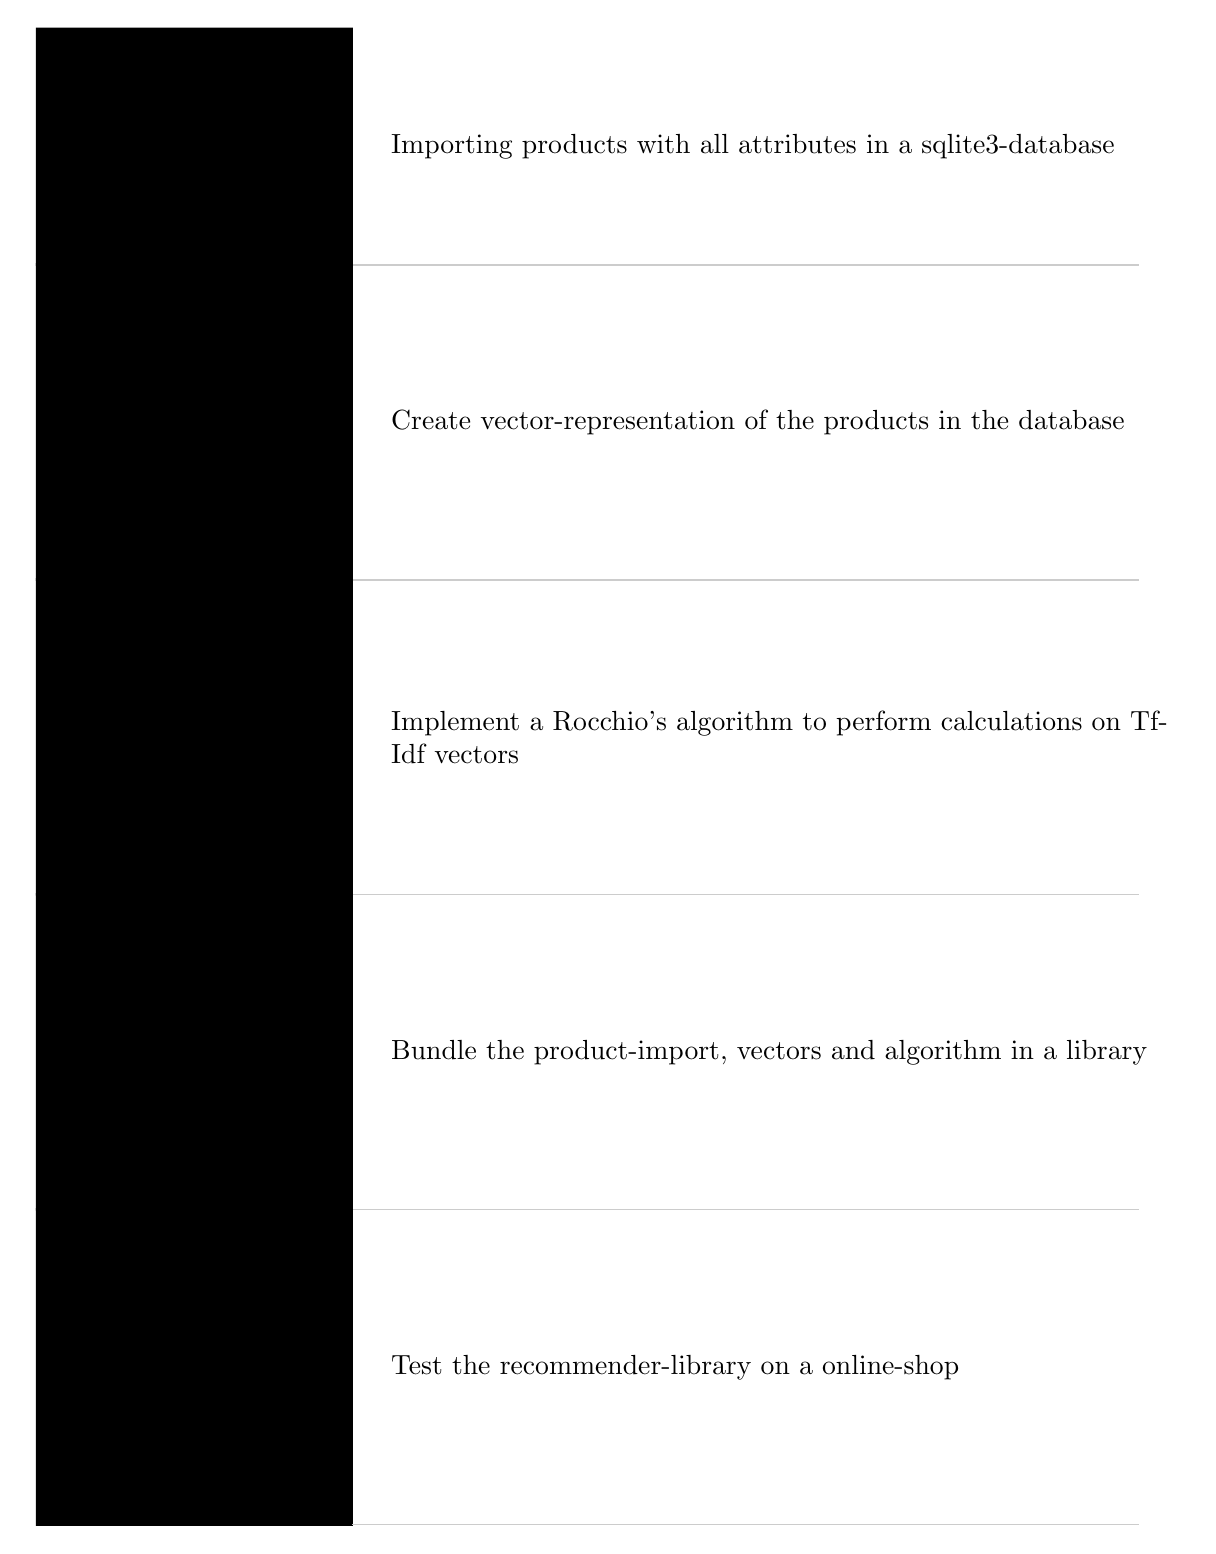
\begin{tikzpicture}
        %\def\dustTempLineWidth{12cm}
        \def\dustTempLineWidth{10cm}
        \def\dustTempNodeWidth{4cm}
        %\def\dustTempNodeHeight{4cm}
        \def\dustTempNodeHeight{3cm}
        \def\dustTempArrowHeight{1cm}
        \def\dustTempYShift{0cm}
        \def\dustTempLineColour{Black!20}

        \def\dustTempYShift{0 * -1 * (\dustTempNodeHeight + \dustTempArrowHeight)}
        \draw[thick,fill=\dustRowFirst]
            (0,0)--(\dustTempNodeWidth /2,-1* \dustTempArrowHeight)--(\dustTempNodeWidth,0)--(\dustTempNodeWidth,\dustTempNodeHeight)--(0,\dustTempNodeHeight)--cycle;
        \node[text width=\dustTempNodeWidth,text centered,yshift=\dustTempYShift] at (\dustTempNodeWidth /2,\dustTempNodeHeight /2)
        {
            \textbf{Import of products}
        };
        \node[text width=\dustTempLineWidth,align=left,yshift=\dustTempYShift] at ({\dustTempNodeWidth + \dustTempLineWidth /2 + 0.5cm},\dustTempNodeHeight/2)
        {
            Importing products with all attributes in a sqlite3-database
        };
        \draw[thin,\dustTempLineColour,yshift=\dustTempYShift] (\dustTempNodeWidth,0)--(\dustTempNodeWidth + \dustTempLineWidth,0);

        \def\dustTempYShift{1 * -1 * (\dustTempNodeHeight + \dustTempArrowHeight)}
        \draw[thick,fill=\dustRowSecond,yshift=\dustTempYShift]
            (0,0)--(\dustTempNodeWidth /2,-1 * \dustTempArrowHeight)--(\dustTempNodeWidth,0)--(\dustTempNodeWidth,\dustTempNodeHeight+\dustTempArrowHeight)--(\dustTempNodeWidth /2,\dustTempNodeHeight)--(0,\dustTempNodeHeight + \dustTempArrowHeight)--cycle;
        \node[text width=\dustTempNodeWidth,text centered,yshift=\dustTempYShift] at (\dustTempNodeWidth /2,\dustTempNodeHeight /2)
        {
            \textbf{Creation of vectors}
        };
        \node[text width=\dustTempLineWidth,align=left,yshift=\dustTempYShift] at ({\dustTempNodeWidth + \dustTempLineWidth /2 + 0.5cm},\dustTempNodeHeight /2 + \dustTempArrowHeight /2)
        {
            Create vector-representation of the products in the database
        };
        \draw[thin,\dustTempLineColour,yshift=\dustTempYShift] (\dustTempNodeWidth,0)--(\dustTempNodeWidth + \dustTempLineWidth,0);

        \def\dustTempYShift{2 * -1 * (\dustTempNodeHeight + \dustTempArrowHeight)}
        \draw[thick,fill=\dustRowFirst,yshift=\dustTempYShift]
        (0,0)--(\dustTempNodeWidth /2,-1 * \dustTempArrowHeight)--(\dustTempNodeWidth,0)--(\dustTempNodeWidth,\dustTempNodeHeight+\dustTempArrowHeight)--(\dustTempNodeWidth /2,\dustTempNodeHeight)--(0,\dustTempNodeHeight + \dustTempArrowHeight)--cycle;
        \node[text width=\dustTempNodeWidth,text centered,yshift=\dustTempYShift] at (\dustTempNodeWidth /2,\dustTempNodeHeight /2)
        {
            \textbf{Implementing recommender algorithm}
        };
        \node[text width=\dustTempLineWidth,align=left,yshift=\dustTempYShift] at ({\dustTempNodeWidth + \dustTempLineWidth /2 + 0.5cm},\dustTempNodeHeight /2 + \dustTempArrowHeight /2)
        {
            Implement a Rocchio's algorithm to perform calculations on Tf-Idf vectors
        };
        \draw[thin,\dustTempLineColour,yshift=\dustTempYShift] (\dustTempNodeWidth,0)--(\dustTempNodeWidth + \dustTempLineWidth,0);

        \def\dustTempYShift{3 * -1 * (\dustTempNodeHeight + \dustTempArrowHeight)}
        \draw[thick,fill=\dustRowSecond,yshift=\dustTempYShift]
        (0,0)--(\dustTempNodeWidth /2,-1 * \dustTempArrowHeight)--(\dustTempNodeWidth,0)--(\dustTempNodeWidth,\dustTempNodeHeight+\dustTempArrowHeight)--(\dustTempNodeWidth /2,\dustTempNodeHeight)--(0,\dustTempNodeHeight + \dustTempArrowHeight)--cycle;
        \node[text width=\dustTempNodeWidth,text centered,yshift=\dustTempYShift] at (\dustTempNodeWidth /2,\dustTempNodeHeight /2)
        {
            \textbf{Create library}
        };
        \node[text width=\dustTempLineWidth,align=left,yshift=\dustTempYShift] at ({\dustTempNodeWidth + \dustTempLineWidth /2 + 0.5cm},\dustTempNodeHeight /2 + \dustTempArrowHeight /2)
        {
            Bundle the product-import, vectors and algorithm in a library
        };
        \draw[thin,\dustTempLineColour,yshift=\dustTempYShift] (\dustTempNodeWidth,0)--(\dustTempNodeWidth + \dustTempLineWidth,0);

        \def\dustTempYShift{4 * -1 * (\dustTempNodeHeight + \dustTempArrowHeight)}
        \draw[thick,fill=\dustRowFirst,yshift=\dustTempYShift]
            (0,0)--(\dustTempNodeWidth,0)--(\dustTempNodeWidth,\dustTempNodeHeight + \dustTempArrowHeight)--(\dustTempNodeWidth /2,\dustTempNodeHeight)--(0,\dustTempNodeHeight + \dustTempArrowHeight)--cycle;
        \node[text width=\dustTempNodeWidth,text centered,yshift=\dustTempYShift]at (\dustTempNodeWidth /2,\dustTempNodeHeight /2)
        {
            \textbf{Set up online-shop}
        };
        \node[text width=\dustTempLineWidth,align=left,yshift=\dustTempYShift] at ({\dustTempNodeWidth + \dustTempLineWidth /2 + 0.5cm},\dustTempNodeHeight /2 + \dustTempArrowHeight /2)
        {
            Test the recommender-library on a online-shop
        };
        \draw[thin,\dustTempLineColour,yshift=\dustTempYShift] (\dustTempNodeWidth,0)--(\dustTempNodeWidth + \dustTempLineWidth,0);

    \end{tikzpicture}

    \caption[Software Milestones]{software milestones}
    \label{fig:softwaremilestones}
\end{figure}

{\color{red}
    Aufgliederung zwischen recherche von state of the art
    und prototyp/impl.



    Ubersicht ueber die Forschugnsfragen
    verweis auf die relevanten textstellen
    beantwortung der Fragen mit explizitem Bezug darauf

    Umschreibung von sec'information retrieval' (kein grosses fass aufmachen)
    zusamenfassen der kapitel IR und Rocchio (evtl. grosses kapitel rocchio mit hinleitung ueber die vectoren)


    Impl >> design and implementation

    Technical details weg lassen (glossary?)


    conclusion
        -summary
            - limitations
        -outlook
}
